\documentclass[14pt, russian, onesize]{extreport}
% BASE
\usepackage[a4paper, margin=0.5in]{geometry}
\usepackage{dingbat} % NICE LINEBREAK
\usepackage{graphicx}
\usepackage{amsmath}
\usepackage{amssymb}
\usepackage{enumitem}
\usepackage{amsfonts}
\usepackage{extarrows}
\usepackage{import}
\usepackage{indentfirst}
\usepackage{caption}
\usepackage{subcaption}
\usepackage{hyperref}
\usepackage{indentfirst}
\usepackage{color}
\usepackage{minted}
\usepackage{enumitem}
% FONTS XeLaTeX
\usepackage[no-math]{fontspec}
\usepackage{mathspec}
\defaultfontfeatures{Ligatures={TeX},Renderer=Basic}
\setmathfont(Digits){Times New Roman}
\setmainfont{Times New Roman}
\setsansfont{Arial}
\setmonofont{Courier New}
\newfontfamily\cyrillicfont[Script=Cyrillic]{Times New Roman}
\newfontfamily\cyrillicfontsf[Script=Cyrillic]{Arial}
\newfontfamily\cyrillicfonttt[Script=Cyrillic]{Courier New}
\usepackage{polyglossia}
\setdefaultlanguage{russian}
% MACRO
\delimitershortfall-1sp
\newcommand\abs[1]{\left|#1\right|}
\definecolor{bg}{rgb}{0.95, 0.95, 0.95}
\newminted{cpp}{ fontsize=\scriptsize, bgcolor=bg, breakafter=, breaklines, breakautoindent=true, breaksymbolleft=\raisebox{0.8ex}{ \small\reflectbox{\carriagereturn}}, breaksymbolright=\small\carriagereturn, }
\newminted{sv}{ fontsize=\small, bgcolor=bg, breakafter=, breaklines, breakautoindent=true, breaksymbolleft=\raisebox{0.8ex}{ \small\reflectbox{\carriagereturn}}, breaksymbolright=\small\carriagereturn, }

\newmintedfile{cpp}{linenos, fontsize=\scriptsize, bgcolor=bg, breaklines, breakafter=,}
\newmintedfile{sv}{linenos,fontsize=\scriptsize, bgcolor=bg, breakafter=, breaklines, breakautoindent=true, breaksymbolleft=\raisebox{0.8ex}{ \small\reflectbox{\carriagereturn}}, breaksymbolright=\small\carriagereturn, }

\newenvironment{code}{\captionsetup{type=listing}}{}

\graphicspath{ {images/} }

\begin{document}
\begin{tabular}{|p{8cm}|p{3cm}|p{3cm}|}
    \hline
    Лабораторная работа №2 & Б10 & 2022\\
    \hline
    Моделирование схем в Verilog  & \multicolumn{2}{|c|}{Хорохорин Андрей Сергеевич}\\
    \hline
\end{tabular}

\section*{ Цель работы }
Построение кэша и моделирование системы <<процессов-кэш память>> на языке описания
Verilog.

\section*{ Инструментарий }
\begin{itemize}
    \item Компилятор \texttt{Icarus Verilog version 11.0 (stable)}
    \item SystemVerilog стандарта \texttt{IEEE1800-2012}
    \item Лучший текстовый редактор \texttt{Vim} с использованием
        \href{https://github.com/dalance/svls?ysclid=lap6k2eu7x964048881}{\color{blue}языкового сервера} \\
        для SystemVerilog
    \item \href{https://github.com/gtkwave/gtkwave?ysclid=lap6sdyzr9924824009}{\color{blue}gtkwave} как средство для просмотра \texttt{.vcd} файлов 
    \item \LaTeX~с расширением \texttt{XeLaTeX} для написания отчёта
\end{itemize}

\section*{ Задача }
Имеется следующее определение глобальных переменных и функций: 
\begin{listing}[H]
    \cppfile[linenos]{listings/task.c}
\end{listing}
\begin{itemize}
    \item Сложение, инициализация переменных и переход на новую итерацию цикла, выход из функции занимают 1 такт.
      Умножение – 5 тактов. Обращение к памяти вида \mintinline{c}{pc[x]} считается за одну команду.
    \item Массивы последовательно хранятся в памяти, и первый из них начинается с 0.
    \item Все локальные переменные лежат в регистрах процессора.
    \item По моделируемой шине происходит только обмен данными (не командами).
\end{itemize}
Необходимо определить процент попаданий 
(число попаданий к общему числу обращений) для кэша и общее время (в тактах),
затраченное на выполнение этой функции.

\newcommand{\var}[1]{\uppercase{\texttt{\textbf{\detokenize{#1}}}}}
\section*{ Вычисление недостающих параметров системы }
\subsection* { Вычисление размера областей памяти }
Везде далее будет считаться, что байт = 8 бит.
Для начала выпишем все параметры кэша и памяти, которые были даны в условии:
\begin{itemize}
    \item \var{cache_way}~--- 2
    \item \var{cache_tag_size}~--- 10 бит
    \item \var{cache_line_size}~--- 16 байт
    \item \var{cache_line_count}~--- 64 линии
    \item \var{mem_size}~--- 512 Кбайт
\end{itemize}

Так как всего в нашем распоряжении \var{cache_line_count}(64) линии,
каждая по \\
\var{cache_line_size}(16 байт), то из них легко вычисляется общий объём полезных
данных, хранимых нашим кэшом. 
\[
    \var{cache_size} = 64 \cdot 16\text{ байт} = 1024\text{ байт } = 1\text{ Кбайт }
\] 

Исходя из того, что всего необходимо проиндексировать 512 Кбайт памяти:
\[
    \var{cache_addr_size} = \lfloor \log_2(512 \cdot 2^{10}) \rfloor = 19\text{ бит}
\]

Исходя из того, что всего у нас \var{cache_line_count}(64) линий и все их нам необходимо
разбить в блоки размера \var{cache_way}(2), то количество блоков 
\[
    \var{cache_sets_count} = 64 / 2 = 32
\]

Для индексации внутри каждого блока будет использоваться \var{cache_offset_size}, поэтому
его размер зависит непосредственно от размера блока \var{cache_line_size}(16 байт)
\[
    \var{cache_offset_size} = \log_2 16 = 4\text{ бит }
\] 

Осталось посчитать размер индекса в наборе кэш-линий \var{cache_set_size}, он должен индексировать
все блоки, которые мы имеем, а их количество нам известно \var{cache_sets_count}(32).
\[
    \var{cache_set_size} = \log_2(32) = 5\text{ бит }
\] 

Заметим, что тег адреса, номер блока и сдвиг внутри блока должен однозначно задавать
адрес ячейки в оперативной памяти, поэтому можно ещё раз проверить верность расчётов,
проверив следующее равенство:
\begin{align*}
    &\var{cache_tag_sz} + \var{cache_set_sz} + \var{cache_offset_sz} = \var{cache_addr_sz}\\
    &10 + 5 + 4 = 19
\end{align*}
Видим, что всё в порядке~--- равенство верно.

Подводя итог, ниже перечислим все необходимые параметры системы:
\begin{itemize}
    \item \var{mem_size}~--- 512 Кбайт
    \item \var{cache_size}~--- 1 Кбайт 
    \item \var{cache_line_size}~--- 16 байт
    \item \var{cache_line_count}~--- 64 линии
    \item \var{cache_way}~--- 2
    \item \var{cache_sets_count}~--- 32 блока
    \item \var{cache_tag_size}~--- 10 бит
    \item \var{cache_set_size}~--- 5 бит
    \item \var{cache_offset_size}~--- 4 бит
    \item \var{cache_addr_size}~--- 19 бит
\end{itemize}
\subsection*{ Вычисление размерности шин }
Начнём с вычисления размера шины адреса между CPU и Cache. В нашей системе обмен
данными по этой шине происходит за два такта. За первый необходимо успеть передать данные
о теге и о номере блока, а за второй~--- offset внутри блока. Больше ни для чего эта
шина не используется, а значит её размер можно сделать следующим:
\begin{align*}
    &\var{addr1_bus_sz}=\max(\var{cache_tag_sz}+\var{cache_set_sz}, \var{cache_offset_sz})\\
    &\var{addr1_bus_sz}=\max(10+5, 4)=15\text{ бит }
\end{align*}

По шине A2 кэш передаёт интересующий его адрес памяти в контроллер памяти, причём
часть адреса offset не передаётся, так как в нашем кэше мы делаем адреса начала кэш
линий кратными их размеру. Так как данная шина ни для чего больше не используется, то
её размер вычисляется следующем образом:
\[
    \var{addr2_bus_sz} = \var{cache_tag_sz} + \var{cache_set_sz} = 10 + 5 = 15\text{ бит }
\]  

Вычисление размерностей шин команд это тривиальная задача, но для неё нам потребуется
вспомнить, какие вообще команды(сигналы) могут передаваться по этим шинам.

\vspace{1cm}
\begin{tabular}{|p{0.45\textwidth}|p{0.45\textwidth}|}
    \hline
\textbf{Cpu $\to$ Cache}
\begin{enumerate}[start=0,label={\arabic*}~---]
    \item \var{c1_nop}
    \item \var{c1_read8}
    \item \var{c1_read16}
    \item \var{c1_read32}
    \item \var{c1_invalidate_line}
    \item \var{c1_write8}
    \item \var{c1_write16}
    \item \var{c1_write32}
\end{enumerate}
&
\textbf{Cpu $\leftarrow$ Cache}
\begin{enumerate}[start=0,label={\arabic*}~---]
    \item \var{c1_nop}
    \addtocounter{enumi}{6}
    \item \var{c1_response}
\end{enumerate}
\\
\hline
\textbf{Cache $\to$ Mem}
\begin{enumerate}[start=0,label={\arabic*}~---]
    \item \var{c2_nop}
    \addtocounter{enumi}{1}
    \item \var{c2_read_line}
    \item \var{c2_write_line}
\end{enumerate}
&
\textbf{Cache $\leftarrow$ Mem}
\begin{enumerate}[start=0,label={\arabic*}~---]
    \item \var{c2_nop}
    \item \var{c2_response}
\end{enumerate}\\
\hline
\end{tabular}
\vspace{1cm}

Из таблицы хорошо видно, что для передачи необходимых сигналов между Cpu и Cache достаточно
3 бит за такт, а для Cache и Mem~--- 2 бита за такт. Таким образом, имеем:
\begin{align*}
    \var{ctr1_bus_sz} = 3\text{ бит }\\
    \var{ctr2_bus_sz} = 2 \text{ бит }
\end{align*}
\newpage
\section*{ Аналитическое решение задачи }
Попытаемся решить задачу аналитически. Для начала немного
более строго сформулировать приведённую в задании систему.
Далее будет считаться, что ни процессор ни кэш не обладают
ни асинхронностью ни параллельностью. То есть когда процессор
отправляет запрос кэшу, он только ждёт ответа и ничего не вычисляет.
То же самое относится и к записи. Помимо этого, в ситуации, когда
кэш ждёт ответа от памяти, он сначала примет все данные от памяти и
только потом начнёт взаимодействие с процессором. То есть
никогда не возникает ситуации, что кэш одновременно общается
по шине и с процессором и с памятью. В ситуации, когда
кэш сообщает памяти новые кэш линии он не ждёт никакого ответа
от памяти. Кроме того, в конце выполнения не обязательно все кэш
линии будут совпадать с памятью, в подсчёте времени работы не
будет закладываться время на то, чтобы полностью синхронизировать
кэш и память с точки зрения того, чтобы ни оказалось ни одной
кэш линии с параметром dirty=1.

Для того, чтобы упростить
себе задачу давайте разделим все такты на два вида: когда процессор
просто ждёт ответа кэша и когда процессор что-то вычисляет. 
Подсчитывать количество попаданий\slash
промахов вручную мне показалось сложным, поэтому был написан 
следующий код, который симулирует работу кэша по модулю того,
что явно не хранит полезные данные и, соответственно,
не возвращает их на запрос.

Тип Word используется для указания количества байт, используемых
при Read\slash Write запросах. Класс CacheLine тоже ничего
умного не делает, это просто удобный контейнер, представляющий
собой кэш-линию, без хранящихся в ней данных.
\begin{cppcode}
typedef unsigned long long Addr;

enum Word { WORD=8, DWORD=16, QWORD=32 };

struct CacheLine {
    const int size;
    bool valid = 0; 
    bool dirty = 0; 
    Addr tag = -1;
    int last_call = 0;
    CacheLine& operator = (CacheLine oth) {
        assert(size == oth.size);
        tie(valid, dirty, tag, last_call) = tie(oth.valid, oth.dirty, oth.tag, oth.last_call);
        return *this;
    }
};
\end{cppcode}

Ниже описан класс, представляющий собой один блок(set) из кэш-линий.
Функции read и write условно эмулируют операцию нашей модели
кэша, при этом read ещё возвращает есть ли запрашиваемый
адрес в блоке или нет. Наверное, самой интересной функцией
является find\_LRO, которая ищет кандидата на вытеснение из
кэша по следующей логике: если есть свободная линия(valid=0),
то вытесняем её, иначе вытесняется линия, к которой условное время
последнего запроса было минимальным. За условное время запроса
берётся просто количество запросов совершенных до этого.
Помимо этого, в классе вычисляется количество
вытесняемый кэш линий, которые необходимо записать в память.
Эта информация пригодится для работы других классов.
\begin{cppcode}

struct CacheSet {
private:
    vector<CacheLine> lines;
    const int line_size;
    int total_mem_pushes = 0;
public:
    CacheSet(int way, int line_size) : line_size(line_size) {
        lines = vector<CacheLine>(way, CacheLine{line_size});
    }

    bool exists(Addr tag) {
        return find_by_tag(tag) != lines.end();
    } 

    void read(Addr tag, int call) {
        auto it = find_by_tag(tag);
        if (it != lines.end()) {
            it->last_call = call;
        } else {
            *(find_LRO()) = CacheLine {line_size, 1, 0, tag, call};
        }
    }

    void write(Addr tag, int call) {
        auto it = find_by_tag(tag);
        if (it != lines.end()) {
            it->last_call = call;
            it->dirty = 1;
        } else {
            total_mem_pushes += find_LRO()->dirty;
            *(find_LRO()) = CacheLine {line_size, 1, 1, tag, call};
        }
    }

    int getMemPushes() const {
        return total_mem_pushes;
    }

private:
    vector<CacheLine>::iterator find_by_tag(Addr tag) {
        return find_if(lines.begin(), lines.end(), [&] (const CacheLine& line) {
                return line.valid && line.tag == tag;
            }
        );
    }

    vector<CacheLine>::iterator find_LRO() {
        return min_element(lines.begin(), lines.end(), [] (const CacheLine& a, const CacheLine& b) {
            return tie(a.valid, a.last_call) < tie(b.valid, b.last_call);
        });
    }
};

\end{cppcode}

Теперь можно перейти к самому сложному классу~--- Cache. Он
занимается тем, что принимает запрос к памяти, определяет
в каком он блоке выполняет его уже на уровне блока. Но помимо
этого он считает интересную нам статистику~--- количество
попаданий в кэш, количество промахов и прогнозируемое общее
время работы данных операций на реальном кэше. Ещё он
считает количество совершённых обращений к памяти в
переменной calls, чтобы 
обеспечивать каждый запрос корректным условным временем.

Стоит отдельно объяснить почему время считается именно таким образом.
В условии задания написано, что, в случае попадания,
первый такт ответа кэша происходит
через 6 тактов после первого такта запроса. Это значит, что 
если данные были переданы за один такт, то на седьмой
такт процессор продолжит исполнять команды, получив ответ
на запрос, который он послал ещё на первом такте. Итого на
одном запросе процессор простаивает 7 тактов. Но данные
от кэша могут передаваться не один такт, поэтому была
сделана внутренняя функция transfer\_lag, которая по порции
данных определяет сколько она будет передаваться.
Так как обе шины данных в нашей системе имеют одинаковую
пропускную способность, эта функция используется для 
аналогичных расчётов при передаче данных от 
памяти к кэшу. 

В случае, когда на кэш поступает запрос записи всё происходит
аналогично чтению за исключением одного момента:
передачи данных от кэша к процессору не происходит,
передаётся только команда-флаг, что всё отработало,
но это всё равно занимает один дополнительный такт.

Помимо всего вышеперечисленного, необходимо помнить, что
когда мы вытесняем из кэша линию, которая помечена dirty=1,
то необходимо послать дополнительный запрос к памяти, эта
поправка вычисляется непосредственно в методе 
get\_time, используя насчитанные значения в каждой из CacheLine.

Также есть <<волшебная>> функция split\_addr,
в которой происходит много битовых операций, чтобы просто 
разбить адрес части на tag, set, offset.
\begin{cppcode}
struct Cache { 
private:
    const int sets_cnt;
    const int way;
    const int line_size;        // byte
    const int data_bus_size;    // bits
    const int mem_size;         // byte

    int total_hits = 0;
    int total_misses = 0;
    int total_time = 0;
    int calls = 0;

    vector<CacheSet> sets;

    struct InnerAddr {
        Addr tag, set, offset;
    };
public:
    Cache(int sets_cnt, int way, int line_size, int data_bus_size, int mem_size) :
        sets_cnt(sets_cnt), way(way), line_size(line_size), data_bus_size(data_bus_size), mem_size(mem_size) {
        sets = vector<CacheSet>(sets_cnt, CacheSet(way, line_size));
    }

    void read(Word word, Addr addr) {
        calls++;
        auto [tag, set, offset] = split_addr(addr); 
        if (sets[set].exists(tag)) {
            total_hits++;
            total_time += 6; // Cache lag
            total_time += transfer_lag(word) + 1; // Cache -> Cpu
                                                  // 8-9
        } else {
            total_misses++;
            total_time += 4 + 100; // Cache + Mem lag
            total_time += transfer_lag(WORD * line_size) + 1; // Mem -> Cache
            total_time += transfer_lag(word); // Cache -> Cpu
                                              // 114-115
        }
        sets[set].read(tag, calls);
    };

    void write(Word word, Addr addr) {
        calls++;
        auto [tag, set, offset] = split_addr(addr); 
        if (sets[set].exists(tag)) {
            total_hits++;
            total_time += 6; // Cache lag 
            total_time += 1; // Cache->Cpu response
        } else {
            total_misses++;
            total_time += 4 + 100;                        // Cache + Mem lag
            total_time += transfer_lag(WORD * line_size); // Mem -> Cache
            total_time += 1; // Cache->Cpu response
        }
        sets[set].write(tag, calls);
    };

    int get_hits() const  {
        return total_hits;
    }

    int get_misses() const {
        return total_misses;
    }

    int get_time() const {
        int total_pushes = accumulate(sets.begin(), sets.end(), 0,
            [] (int acc, const CacheSet& el) {
                return acc + el.getMemPushes();
            }
        );
        return total_time + total_pushes * (100 + 1);
    }

private:
    InnerAddr split_addr(Addr addr) const {
        return {
            (addr & ((mem_size - 1) & ~(sets_cnt * line_size - 1))) / (sets_cnt * line_size),
            (addr & (sets_cnt - 1) * line_size) / line_size ,
            addr & (line_size - 1)
        };
    }

    int transfer_lag(int data) const {
        return (data + data_bus_size - 1) / data_bus_size;
    }

};
\end{cppcode}

Теперь давайте направим всё реализованное нами <<чудо>> на решение задачи.
Код ниже не симулирует пример из задачи полностью, а лишь обращается
с запросами чтения\slash записи
к тем же адресам, но для анализа времени работы кэша это и требуется.
Класс PseudoAllocator просто помогает симулировать
последовательное выделение памяти для массивов, возвращая 
адреса начала каждого из них.

\begin{cppcode}
struct PseudoAllocator {
    Addr last_allocated_addr = 0;
    
    Addr allocate(int n, int m, int elem_sz) {
        int res = last_allocated_addr;
        last_allocated_addr += n * m * elem_sz;
        return res;
    }
};

int main() {
    // 512Kb == [0x00000...0x7ffff]
    Cache cache(32, 2, 16, 16, 512 * 1024);
    PseudoAllocator alloc;

    const int M = 64;
    const int N = 60;
    const int K = 32;

    int8_t*  a = (int8_t*) alloc.allocate(M, K, sizeof(int8_t));  // a[M][K];
    int16_t* b = (int16_t*)alloc.allocate(K, N, sizeof(int16_t)); // b[K][N];
    int32_t* c = (int32_t*)alloc.allocate(M, N, sizeof(int32_t)); // c[M][N];

    for (int y = 0; y < M; y++) {
        for (int x = 0; x < N; x++) {
            int16_t* pb = b;
            for (int k = 0; k < K; k++) {
                cache.read(WORD, (Addr) (a + k));
                cache.read(DWORD, (Addr) (pb + x));
                pb += N;
            }
            cache.write(QWORD, (Addr) (c + x));
        }
        a += K;
        c += N;
    }

    cout << "HITS: " << cache.get_hits() << "\nMISSES: " << cache.get_misses() << "\nTOTAL TIME: " << cache.get_time() << endl;
    cout << "RATE: " << 1.0 * (cache.get_hits()) / (cache.get_hits() + cache.get_misses()) << endl;

    return 0;
}
\end{cppcode}
Ниже приведён вывод данного кода:\\
\texttt{
HITS: 228080\\
MISSES: 21520\\
TOTAL TIME: 4274080\\
RATE: 0.913782\\
}
Теперь, когда мы знаем за сколько работает кэш, вычислим время
работы всего остального. 
\begin{itemize}
    \item 
        Один такт на выход из функции.
    \item 
        Инициализация переменных, каждая из которых выполняется
        за один такт. Она явно выполняется в строчках 9, 10, 13, 14. 
        И неявно в каждом из циклов. Будем считать, что переменные локальные
        для цикла выделяются заново на каждой итерации внешнего цикла.
        Тогда суммарное количество инициализаций вычисляется как: 
        $3 + M + M \cdot N \cdot 3 = 11587$ 
    \item 
        Подсчитаем количество тактов на сложение, включив в них
        такты на смену итерации цикла. 
        $M \cdot 3+ M \cdot N + M \cdot N \cdot K \cdot 3 = 372672$
    \item 
        Количество тактов на умножение: 
        $M \cdot N \cdot K \cdot 5 = 614400$ 
\end{itemize}
Итого дополнительно имеем: $1 + 11587 + 372672 + 614400 = 998660$.
Тогда итоговое прогнозируемое время работы равно:
$998660 + 4274080 = 5272740$

\section*{ Моделирование на языке Verilog }
\subsection*{ Структура проекта }
Стоит начать с общей структуры модели и с её организации на
файлы. Логически есть 3 модуля: процессор, кэш и память,
причём процессор в нашем случае не был реализован явно, а лишь в
тестового окружения на Verilog, который лишь 
симулирует работу настоящего процессора для кэша.

Пройдёмся по файлам: 
\begin{itemize}
    \item 
        \texttt{parameters.sv} для описания глобальных констант
        и структур.
    \item
        \texttt{clock.sv} в котором задаётся
        модуль \texttt{Clock}, который используется
        для синхронизации схем и оценки времени их работы, так как
        внутри себя он считает количество тактов.
    \item 
       \texttt{cache.sv} и \texttt{mem.sv} задают основные 
       модули данного проекта~--- \texttt{Cache} и \texttt{Memory}. Отдельно
       стоит отметить, что в этих же файлах располагаются
       удобные интерфейсы доступа к ним: \texttt{CacheDriver, MemoryDriver}.
       Они необходимы для избежания дублирования кода, так как
       к кэшу и к памяти есть нужда обращаться из разных
       модулей, а писать больше одного раза код, который 
       описывает протокол общения с кэшом очень непродуктивно. 
    \item 
        \texttt{mem\_testbench.sv} и \texttt{cache\_testbench.sv}
        хранят реализацию модулей Unit тестов для памяти и кэша 
        соответственно.
        Помимо корректности, они проверяют ещё и время работы 
        модулей в различных ситуациях, что оказалось чрезвычайно полезным.
\end{itemize}

Для подключения модулей используется директива \mintinline{sv}{include}, работающая
аналогично одноимённой директиве в C и имеющая те же проблемы: а именно
множественный include одного и того-же модуля и, как следствие,
ошибка компиляции. В Verilog эта проблема решается точно
так как, как и в C, при помощи так называемых include guards.
\begin{svcode}
`ifndef CPU_GUARD
`define CPU_GUARD
...
`endif
\end{svcode}

\subsection*{ Inout шины }
Поясним, как реализованы inout шины на Verilog. Для примера
возьмём часть кода из файла \texttt{mem.sv}, в которой
реализована шина адреса \texttt{cmd\_w}.
\begin{svcode}
module Memory
    (
        inout wire[1:0] cmd_w
    );

    bit owner = 0;
    logic[1:0] cmd;

    assign cmd_w = owner ? cmd : 2'bzz;

\end{svcode}
Для каждой шины в модуле 
заводится bit переменная обозначающая, владеет ли данный модуль
шиной в текущий момент времени. В данном примере она названа \texttt{owner}.
Помимо этого, каждый \mintinline{sv}{inout} 
выход модуля имеет logic переменную внутри модуля, данном
случае это \texttt{cmd}. Она необходима
для того, чтобы взаимодействовать с шиной \texttt{cmd\_w} как output,
так как напрямую записать значение в неё не получится. Поэтому
делается интересный трюк при помощи конструкции\\
\mintinline{sv}{ assign cmd_w = owner ? cmd : 2'bzz },
которая в конце каждого такта присваивает значение \texttt{cmd\_w}
либо \texttt{cmd}, если наш модуль должен выставлять значение
на шине, либо высокоимпедансное состояние для того, чтобы
на проводках \texttt{cmd\_w} принимались значения, которые 
выставляет другая сторона и не появлялось конфликтов сигналов,
которые могут реальной схеме даже привести к короткому замыканию
и натурально поджарить нашу схему. 

Так как описанный выше трюк приходится осуществлять с любой
шиной, работающей на ввод-вывод, то эти подробности реализации
помещены в модули-драйверы, для удобства моделирования вышестоящих
уровней.
\subsection*{ Почему размер шин адреса не совпадает с минимальным достаточным? }
Отдельно хочу отметить, что размер шин адреса 
\var{addr1_bus_size} и\\ \var{addr2_bus_size} в моей реализации
округлены до 16, для того, чтобы все шины адреса и данных единообразно
задавались целым количеством байт, мне показалось это удобным программировать.

В действительности, если бы я писал код заново, лучшим решением было бы
хранить все размеры в битах.
\subsection*{ Функция skip }
Почти в каждом модуле можно видеть следующую функцию, которая
необходима для удобного программирования схемы.
\begin{svcode}
    task automatic skip(input longint ticks = 1);
        logic enter_clk = clk;
        while (ticks > 0) begin
            wait(clk != enter_clk);
            wait(clk == enter_clk);
            ticks--;
        end
    endtask
\end{svcode}
Стоит отметить, что очень важным является то, что она
ждёт не posedge\slash negedge, а именно такт, то есть
данная функция не меняет чётности синхронизации. Это
очень важно и много где используется.
К сожалению, я не нашёл и не придумал способа не дублировать
её код в каждом из модулей, так как если передавать clk по\\
\mintinline{sv}{input logic clk} аргумент, то он не будет
обновляться внутри этой функции. Действительно в стандарте
SystemVerilog на этот случай есть \mintinline{sv}{ref logic clk},
что делало ровно то, что нам надо, но эта конструкция не 
поддерживается в \texttt{Icarus Verilog 11}, поэтому от
её использования пришлось отказаться. 

\subsection*{ Про выравнивания структур }
Стоит обратить внимание на ключевое слово \mintinline{sv}{packed} 
в объявлениях структур. Выглядит это примерно так:
\begin{svcode}
    typedef struct packed { 
        logic[cache_tag_size-1:0] tag;
        logic[cache_set_size-1:0] set;
        logic[cache_offset_size-1:0] offset;
    } cacheAddr;
\end{svcode}

Такая конструкция гарантирует, что все данные структуры будут
расположены последовательно, без каких-либо пропусков. Это позволяет
значительно упростить себе присваивание значений для этой структуры,
пользуясь конструкциями, описанными в следующем пункте.

\subsection*{ Проблемы при записи в структуру }
Из-за особенностей Verilog в массиве структур нельзя изменить
отдельное поле, в этом случае при компиляции выдаётся следующая ошибка.\\
\texttt{
error: Array index expressions must be constant here.
}\\
Это решается тем, что записывать структуру целиком можно, это выглядит
так: 
\begin{svcode}
    lines[it] <= {1'b1, 1'b1, total_hits + total_misses, curAddr.tag, buff_b};
\end{svcode}
В коде выше, конструкция с перечислением внутри фигурных скобок называется
concatenation operator, и занимается тем, что конкатенирует всё
внутри в один регистр \mintinline{sv}{logic}. Интересным
моментом является то, как написаны константы \mintinline{sv}{1'b1},
эта запись позволяет задаёт число в виде регистра заданной длины. В 
противном случае, запись \mintinline{sv}{1} представляла бы собой 
регистра размера 32 и вся запись в структуру бы <<поплыла>>. 
\subsection*{ Про блокирующие и неблокирующие присваивания }
В коде выше используется нестандартное присваивание, которое называется
неблокирующим. Оно применяется не сразу, а только в самом конце текущего
такта, что позволяет делать следующие трюки. Вот код, который за такт
меняет значение переменных a и b местами.
\begin{svcode}
    a <= b;
    b <= a;
\end{svcode}

Его использование предохраняет от состояния <<гонки>> присвоения,
так как гораздо проще спрогнозировать поведение несколько присвоений, 
которые происходят одновременно, чем нескольких последовательных.
Помимо этого, код в котором меньше блокирующих присваиваний будет
лучше преобразовываться в реальную схему.

В моей программе, я старался
придерживаться следующей логики: переменные, которые используются
для внутренней логики модуля и никак не взаимодействуют
с другими модулями используют блокирующие присваивание, а значения
на шинах и всё, что с ними связано~--- неблокирующее. 

\subsection*{ Протоколы взаимодействия модулей }
\subsubsection*{ Протокол работы с кэшом }
При чтении из кэш у меня реализована следующая схема. На первом и 
втором такте передачи кэшу передаётся адрес, после чего
владение шиной переходит кэшу. Спустя некоторое время, кэш
на высокой синхронизации посылает значение \var{C1_RESPONSE}, одновременно
с этим начиная передавать данные. 

На схемах нарисован график синхронизации, на верхних
значениях которого написаны действия кэша , а на нижних, соответственно,
процессора в каждый такт синхронизации. 
Пунктирной линией обозначена смена владельца шины.
В коде это реализовано таким образом, что процессор отрабатывает
сразу после \mintinline{sv}{@(posedge clk)}, а кэш наоборот,
сразу после \mintinline{sv}{@(negedge clk)}. Исключением из этого
правила служит передача доступа от одной стороне другой, в этом случае
сторона, которая прекращает владеть шиной, должна сообщить это не в свой
такт, но в этот факт она просто снимает с себя владение шиной и ничего больше.

Приношу извинения за картинки от руки,
inkscape неожиданно отказался работать должным образом. 
\begin{figure}[H]
    \centering
    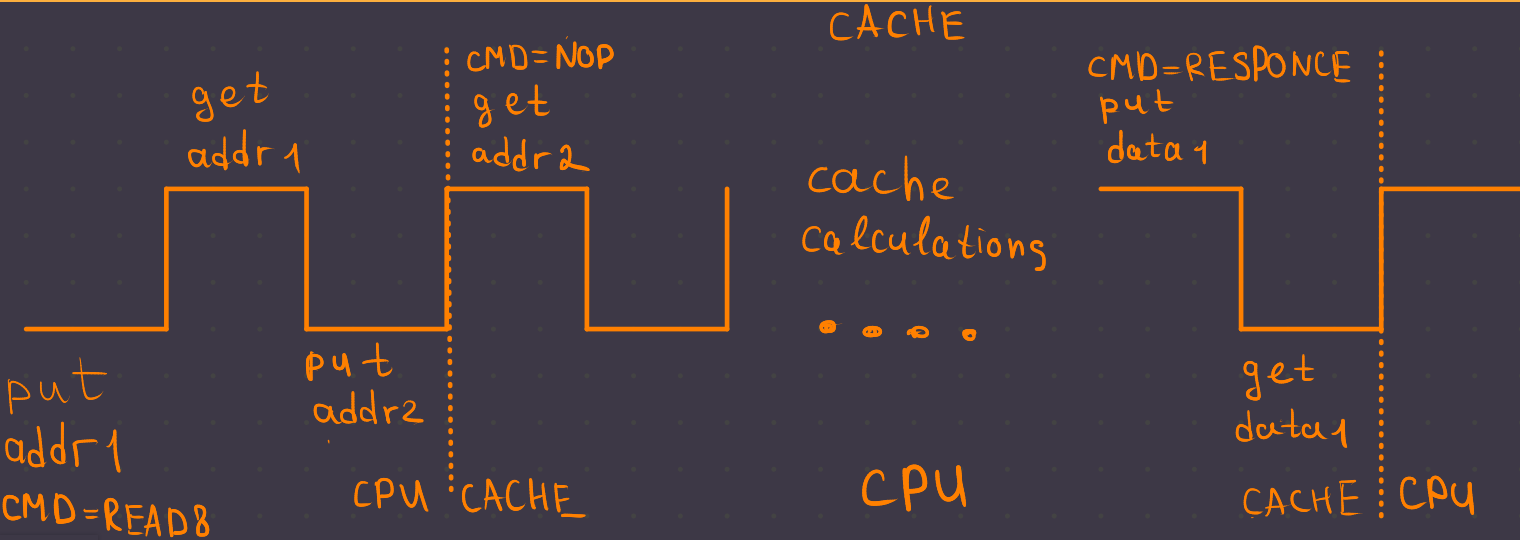
\includegraphics[width=0.9\textwidth]{cache_read}
    \caption{\var{C1_READ8}}
\end{figure}

При запросе записи всё проходит почти аналогично. Обратите внимание,
тут данные тоже передаются не сразу, а с задержкой в один такт от адреса.
Позже оказалось, что это самое удачное решение,
ведь мы тратим лишний такт, но решил всё таки оставить так.
\begin{figure}[H]
    \centering
    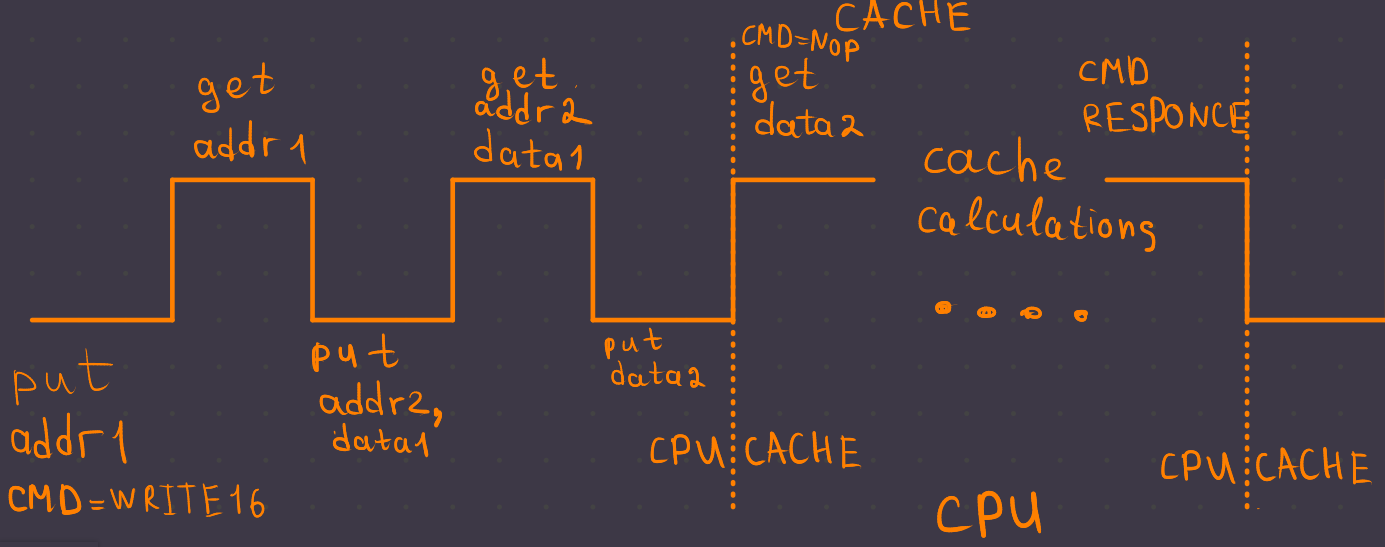
\includegraphics[width=0.9\textwidth]{cache_write}
    \caption{\var{C1_WRITE16}}
\end{figure}

\subsubsection*{ Протокол работы памятью }
В ней всё очень похоже на работу кэша, но на всякий случай 
приведу схемы и для памяти. Сверху обозначены действия памяти,
а снизу~--- кэша.
\begin{figure}[H]
    \centering
    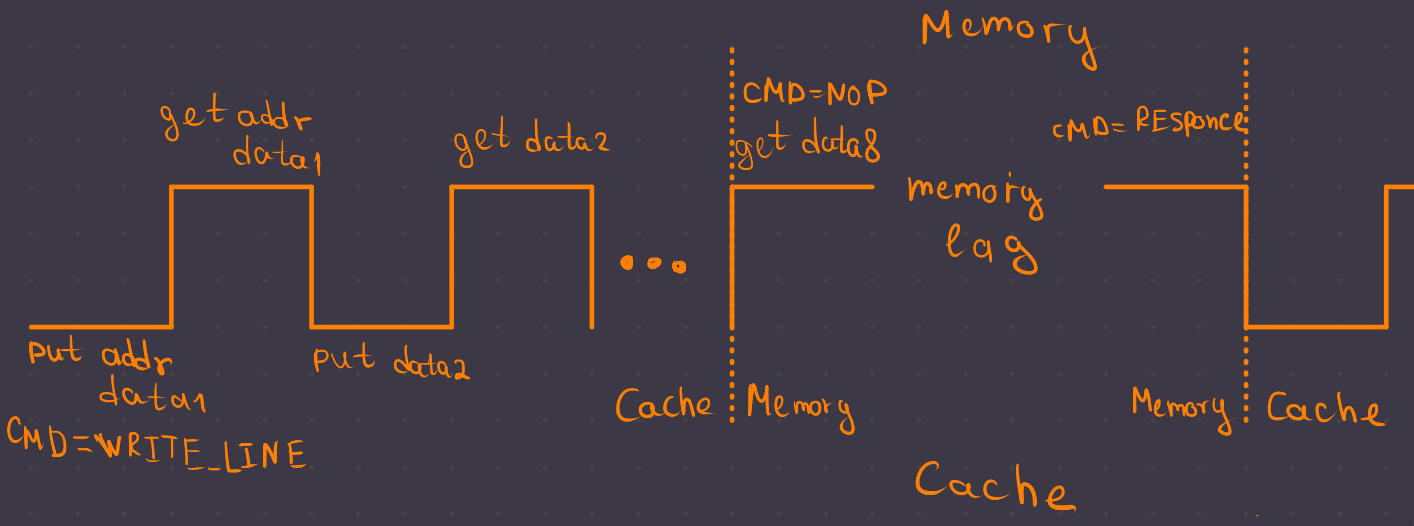
\includegraphics[width=0.9\textwidth]{memory_write}
    \caption{\var{C2_WRITELINE}}
\end{figure}

\begin{figure}[H]
    \centering
    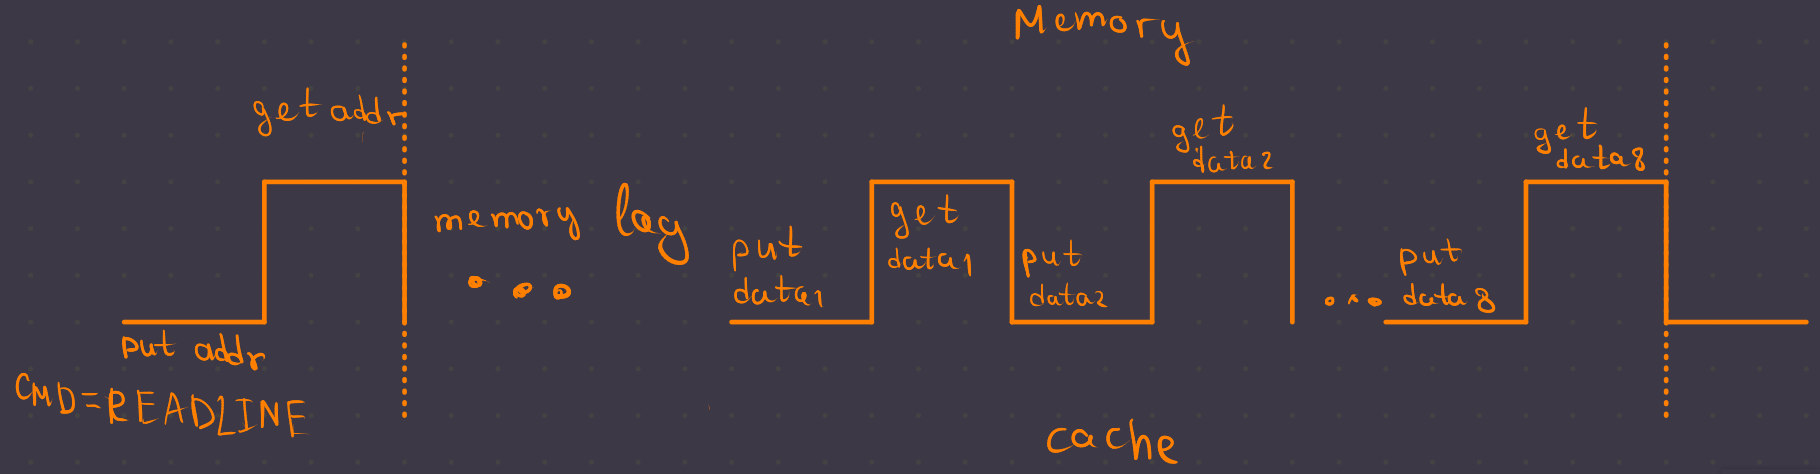
\includegraphics[width=0.9\textwidth]{memory_read}
    \caption{\var{C2_READLINE}}
\end{figure}
Для наглядности также привету код для считывания памяти c обеих сторон.
\begin{svcode}
    // Memory
    always @(posedge clk) begin
        if (cmd_w == C2_READ_LINE) begin
            cmd <= C2_NOP;
            owner <= 1;
            skip(mem_feedback_time - 1);
            @(negedge clk)
            cmd <= C2_RESPONSE;
            for (it = addr * cache_line_size; it < addr * cache_line_size + cache_line_size; it += data2_bus_size) begin
                for (byte_in_bus = 0; byte_in_bus < data2_bus_size; byte_in_bus += 1) begin
                    data[byte_in_bus * BITS_IN_BYTE +: BITS_IN_BYTE] <= heap[it + byte_in_bus];
                end
                if (it + data2_bus_size >= addr * cache_line_size + cache_line_size)
                    @(posedge clk);
                else
                    @(negedge clk);
            end
            owner <= 0;
        end
    end
    // Cache
    task run_read(input logic[cache_set_size + cache_tag_size-1:0] addr_, output logic[cache_line_size*BITS_IN_BYTE-1:0] data_, output longint timing);
        @(negedge clk);
        owner <= 1;
        cmd <= C2_READ_LINE;
        addr <= addr_;
        timing = clk_time;
        @(posedge clk);
        owner <= 0;
        wait(cmd_w == C2_RESPONSE); 
        @(posedge clk);
        timing = clk_time - timing;
        for (i = 0; i < cache_line_size; i += data2_bus_size) begin
            data_[i * BITS_IN_BYTE +: data2_bus_size * BITS_IN_BYTE] <= data_w;
            if (i + data2_bus_size >= cache_line_size)
                @(negedge clk);
            else
                @(posedge clk);
        end
        owner <= 1;
        cmd <= C2_NOP;
    endtask
\end{svcode}

\section*{ Воспроизведение задачи на Verilog }
В файле \texttt{testbench.sv} задано тестовое окружение для данной 
задачи, в котором выводится интересная статистика. В неё
входит общее количество тактов работы задачи, количество
тактов, затраченное на работу кэша, количество попаданий
и промахов в кэш, а также время работы после каждой
итерации внешнего цикла. 

\begin{svcode}
    for (y = 0; y < M; y++) begin skip(); // loop
        skip(); // x init;
        ...
        ...
        $display("time: %d %t", y, timing);
        $fflush;
    end
    
    $display("Finish cpu run");
    $display("Time: %t", timing);
    $display("Cache time: %t", timing - skipped_time);
    $display("Alu time: %t", skipped_time);
    $display("Total hits: %d", total_hits);
    $display("Total misses: %d", total_misses);
    $finish;
\end{svcode}

Результат работы:\\
\texttt{
time:           0                83637\\
...\\
time:          62              5191123\\
time:          63              5272741\\
Finish cpu run                        \\
Time:              5272742            \\
Cache time:              4274080      \\
Alu time:               998662        \\
Total hits:      228080               \\
Total misses:       21520             \\
}

\section*{ Сравнение полученных результатов }
Изначально прогнозированное время работы было меньше реально примерно на 20\%.
Это произошло главным образом из-за плохой реализации передачи данных по шине. 

В коде на Verilog много где была сформирована модель, что
принимающая сторона синхронизируется по \mintinline{sv}{posedge clk},
а отдающая по \mintinline{sv}{negedge clk} или наоборот.
Из-за этого очередная операция считывания могла быть начата
на такт позже из-за того, что на данном такте \mintinline{sv}{negedge clk},
а эта схема синхронизируется по \mintinline{sv}{posedge clk} перед отправкой.

Но описанная выше проблема была исправлена после исправления не оптимальных мест
и изменения логики синхронизации. В этом мне очень помогли написанные тесты.
После этих изменений, время, полученное во время
симуляции кода на Verilog в точности совпало с прогнозом.

\section*{ Листининг кода }
\subsection*{ Код на C++ для оценки времени работы }
\begin{code}
    \cppfile{listings/cpp/main.cpp}
    \caption{main.cpp}
\end{code}
\subsection*{ Код на Verilog для симуляции схемы }
\begin{code}
    \svfile{listings/verilog/parameters.sv}
    \caption{parameters.sv}
\end{code}
\begin{code}
    \svfile{listings/verilog/clock.sv}
    \caption{clock.sv}
\end{code}
\begin{code}
    \svfile{listings/verilog/mem.sv}
    \caption{mem.sv}
\end{code}
\begin{code}
    \svfile{listings/verilog/cache.sv}
    \caption{cache.sv}
\end{code}
\subsection*{ Код тестирования в среде Verilog }
\begin{code}
    \svfile{listings/verilog/testbench.sv}
    \caption{testbench.sv}
\end{code}
\begin{code}
    \svfile{listings/verilog/mem_testbench.sv}
    \caption{mem\_testbench.sv}
\end{code}
\begin{code}
    \svfile{listings/verilog/cache_testbench.sv}
    \caption{cache\_testbench.sv}
\end{code}
\end{document}
